\makeatletter
\def\input@path{{./}{../}{../../}{../../../}{../../../../}{preamble/}{../preamble/}{../../preamble/}{../../../preamble/}}
\makeatother
\input{preamble_exams.tex}
\input{graphs/highlights.tex}
% \GTenHighlightsfalse % Uncomment to disable instructional highlights.
\input{graphs/specific_highlights.tex}

\hypersetup{pdftitle={Grade 10 Global Economics: Term 3, Lesson 1, C4},pdfsubject={Home practice: Empirical Data and Continuous Models}}
\title{Grade 10 Global Economics\\Term 3, Lesson 1: Home Practice\\C4 --- Empirical Data and Continuous Models}
\author{}
\date{}
\begin{document}
\maketitle
\setcounter{tocdepth}{1}
\setcounter{secnumdepth}{2}
\phantomsection\label{toc}
\tableofcontents
\section*{Evaluated criteria}
\begin{description}
\item[\textbf{C4}] Uses frequency distributions, quartiles, percentiles, and graphical representations to describe empirical economic data and compare its shape, centre, and spread with a continuous probability model.
\end{description}
\textbf{How to practise.} Order the observations and keep counts, relative frequencies and model probabilities separate. Use the stated rank convention throughout and label every graph axis. Try each task on paper before opening its solution link. Record the model, working, units and an interpretation; use the arrows to return.
All datasets and economic or financial models in this activity are illustrative, rather than observed market evidence.

\clearpage
\section{Introduction}\label{sec:introduction}
\subsection*{Highlight legend}
\phantomsection\label{tab:highlight-legend}
\begin{tabularx}{\linewidth}{@{}>{\raggedright\arraybackslash}p{.20\linewidth}>{\raggedright\arraybackslash}p{.22\linewidth}>{\raggedright\arraybackslash}X@{}}
\toprule
\textbf{Symbol or notation} & \textbf{Concept} & \textbf{Brief meaning}\\
\midrule
$f_i,\ \HLSampleProportion{f_i/n}$ & \HLSampleProportion{Relative frequency} & Observed fraction in a class. \\
$\HLSampleMean{\bar x}$ & \HLSampleMean{Sample mean} & Average of the data. \\
$Q_1,\ Q_2,\ Q_3$ & Quartiles & Quarter-position summaries. \\
$P_k,\ \mathrm{IQR}$ & Percentile and spread & Rank cutoff and middle-half width. \\
$\HLProbability{P(X\in I)}$ & \HLProbability{Model probability} & Theoretical area for a band. \\
\bottomrule
\end{tabularx}
\subsection{Introductory example 1: A small sample of delivery charges}\label{ex:intro-one}
An illustrative ordered sample of delivery charges is $2,3,4,5,6,7,8,9$ dollars. Its \HLSampleMean{sample mean} is $\HLSampleMean{\bar x=5.5}$ dollars. The \GTenHLSecond{median} is $(5+6)/2=5.5$ dollars. These describe observed charges; a model for future charges is an additional assumption.
\subsection{Introductory example 2: A model and a sample proportion}\label{ex:intro-two}
For the eight charges, two are at most three dollars, giving an \HLSampleProportion{empirical relative frequency} of $\HLSampleProportion{2/8=0.25}$. Under a separate model $X\sim U(2,10)$, the \HLProbability{model probability} below three dollars is $\HLProbability{(3-2)/8=0.125}$. Sample frequencies need not equal model areas.
\section{Notation Reference and Practice Procedure}\label{sec:notation-and-procedure}
\subsection{Notation reference}\label{tab:notation-reference}
\begin{tabularx}{\linewidth}{@{}>{\raggedright\arraybackslash}p{.16\linewidth}>{\raggedright\arraybackslash}p{.18\linewidth}>{\raggedright\arraybackslash}p{.27\linewidth}>{\raggedright\arraybackslash}X@{}}
\toprule
\textbf{Symbol or notation} & \textbf{Concept} & \textbf{Definition} & \textbf{Meaning in the introductory examples}\\
\midrule
$f_i,\ \HLSampleProportion{f_i/n}$ & \HLSampleProportion{Relative frequency} & $f_i$ counts observations; dividing by sample size $n$ gives an observed proportion. & \textbullet\ \hyperref[ex:intro-two]{Example 2}: Two of eight charges are at most three dollars. \\
$\HLSampleMean{\bar x}$ & \HLSampleMean{Sample mean} & Sum of all observed values divided by $n$. & \textbullet\ \hyperref[ex:intro-one]{Example 1}: Average charge is 5.5 dollars. \\
$Q_1,\ Q_2,\ Q_3$ & Quartiles & Here $Q_2$ is the usual median; $Q_1=P_{25}$ and $Q_3=P_{75}$ use the nearest-rank rule below. & \textbullet\ \hyperref[ex:intro-one]{Example 1}: Ordered charges locate quarter positions. \\
$P_k,\ \mathrm{IQR}$ & Percentile and spread & $P_k=x_{(lceil kn/100
ceil)}$ for $0<kle100$; $mathrm{IQR}=Q_3-Q_1$. & \textbullet\ \hyperref[ex:intro-one]{Example 1}: The data have eight ordered positions. \\
$\HLProbability{P(X\in I)}$ & \HLProbability{Model probability} & A continuous density gives interval probability as area, rather than an observed count. & \textbullet\ \hyperref[ex:intro-two]{Example 2}: The uniform model gives 0.125 below three dollars. \\
\bottomrule
\end{tabularx}
\subsection{Practice procedure}
\begin{enumerate}
\item Identify the sample, units and sample size. Order raw data or build a complete frequency table with nonoverlapping classes.
\item Compute relative and cumulative frequencies. Use exact observations for ranks when available; grouped intervals may only locate a percentile class.
\item State the median, percentile and quartile convention, then find centre and spread. Draw a histogram and/or box plot with units.
\item Compare empirical proportions and graph shape with specified model areas, centre and spread. Describe differences without treating a small sample as proof of a model.
\end{enumerate}
\subsection{Conventions used in every task}
For ordered data $x_{(1)}\le\cdots\le x_{(n)}$, the median averages the two central values when $n$ is even. All other requested percentiles use \textbf{nearest rank}: rank $r=\lceil kn/100\rceil$ for $P_k$. Set $Q_1=P_{25}$ and $Q_3=P_{75}$, so the quartiles are not computed by a different half-sample convention. The range is maximum minus minimum. A box plot uses minimum, $Q_1$, median, $Q_3$, maximum with full-range whiskers here. For equal-width histograms, bar heights may show frequencies; comparisons with density curves require relative-frequency density $f_i/(n\,w_i)$ instead. Classes are left-closed, right-open unless the final endpoint is explicitly included.
\section{General Worked Problems}\label{sec:general-worked}
\SectionProblemsTableOfContents{
\SectionProblemLink{prob:sec:general-worked0}{From raw costs to a graph}\\
\SectionProblemLink{prob:sec:general-worked1}{Comparing data with a uniform model}\\
\SectionProblemLink{prob:sec:general-worked2}{What a grouped table can reveal}}

\subsection{From raw costs to a graph}\label{prob:sec:general-worked0}
The complete illustrative sample of twelve delivery costs, in dollars, is
\[
2,\ 3,\ 4,\ 4,\ 5,\ 5,\ 6,\ 6,\ 7,\ 8,\ 9,\ 13.
\]
Use classes $[2,5)$, $[5,8)$, $[8,11)$ and $[11,14]$.
\QuestionsTasks[sec:general-worked]{{4}/{sol:sec:general-worked0}/{Construct frequency and cumulative-frequency tables. Find the mean, median, quartiles, interquartile range and 90th percentile. Describe a histogram and draw a box plot.}}
\subsubsection*{Worked solution}\label{sol:sec:general-worked0}
The data are already ordered. Counting every observation once gives
\[
\begin{array}{c|rrrr}
\text{Cost class (dollars)} &[2,5)&[5,8)&[8,11)&[11,14]\\ \hline
f_i&4&5&2&1\\
f_i/12&4/12&5/12&2/12&1/12\\
\text{Cumulative count}&4&9&11&12
\end{array}
\]
The sum is $82$ dollars, so $\HLSampleMean{\bar x}=82/12=41/6\approx6.83$ dollars. The median is $(5+6)/2=5.5$ dollars. Nearest ranks are $\lceil0.25(12)\rceil=3$ and $\lceil0.75(12)\rceil=9$, giving $Q_1=4$, $Q_3=7$ and $\mathrm{IQR}=7-4=3$ dollars. Rank $\lceil0.90(12)\rceil=11$ gives $P_{90}=9$ dollars. The range is $13-2=11$ dollars.
\begin{center}
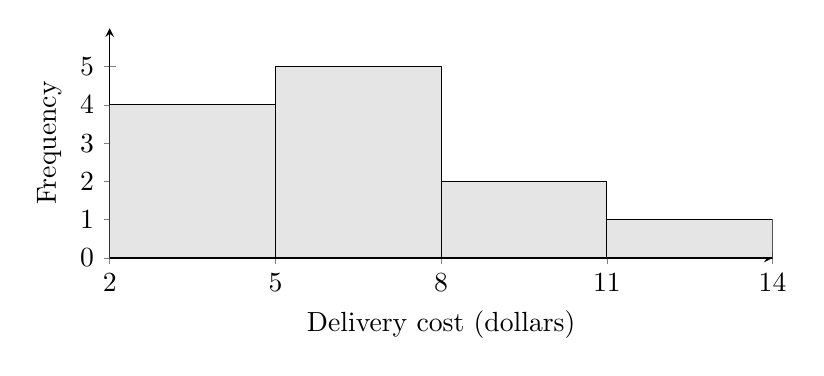
\begin{tikzpicture}
\begin{axis}[width=10cm,height=4.5cm,axis lines=left,xlabel={Delivery cost (dollars)},ylabel={Frequency},xmin=2,xmax=14,ymin=0,ymax=6,xtick={2,5,8,11,14},ytick={0,1,2,3,4,5}]
\addplot[draw=black,fill=gray!20] coordinates {(2,0)(2,4)(5,4)(5,0)} \closedcycle;
\addplot[draw=black,fill=gray!20] coordinates {(5,0)(5,5)(8,5)(8,0)} \closedcycle;
\addplot[draw=black,fill=gray!20] coordinates {(8,0)(8,2)(11,2)(11,0)} \closedcycle;
\addplot[draw=black,fill=gray!20] coordinates {(11,0)(11,1)(14,1)(14,0)} \closedcycle;
\end{axis}
\end{tikzpicture}
\end{center}
The longer right tail and mean above the median suggest right skew. A full-range box plot is:
\begin{center}\begin{tikzpicture}[x=.65cm,y=.6cm]
\draw[->] (1,0)--(14,0) node[right]{dollars};
\foreach \x in {2,4,7,13}{\draw (\x,.1)--(\x,-.1) node[below]{$\x$};}
\draw (2,1)--(4,1) (7,1)--(13,1);
\draw (2,.6)--(2,1.4) (13,.6)--(13,1.4);
\draw (4,.5) rectangle (7,1.5);
\draw (5.5,.5)--(5.5,1.5) node[above]{$5.5$};
\end{tikzpicture}\end{center}
The long upper whisker describes the large observed charge without assuming a normal distribution.
\secInicio[prob:sec:general-worked0][sec:general-worked]


\subsection{Comparing data with a uniform model}\label{prob:sec:general-worked1}
Use the twelve raw costs from the preceding problem, repeated here for convenience: $2,3,4,4,5,5,6,6,7,8,9,13$ dollars. A proposed model is $X\sim U(2,14)$.
\QuestionsTasks[sec:general-worked]{{4}/{sol:sec:general-worked1}/{Compare empirical and modeled proportions below eight dollars, median, quartiles, range and histogram shape. Discuss whether matching a range establishes a good fit.}}
\subsubsection*{Worked solution}\label{sol:sec:general-worked1}
There are nine observed costs below eight dollars, so the \HLSampleProportion{empirical proportion} is $\HLSampleProportion{9/12=0.75}$. The model's rectangle gives
\[
P(X<8)=\frac{8-2}{14-2}=\HLProbability{0.50}.
\]
The uniform model has centre $(2+14)/2=8$ dollars, quartiles $2+0.25(12)=5$ and $2+0.75(12)=11$, and IQR $6$ dollars. The empirical median is $5.5$ dollars, quartiles are $4$ and $7$, and IQR is $3$ dollars. Its range is $11$ dollars, while the model support width is $12$ dollars.
The model assigns $0.25$ to each three-dollar class. Its density height is $1/12$ per dollar; empirical density heights are $4/36,5/36,2/36,1/36$. These areas reproduce the relative frequencies, so they can be compared with the model on the same scale. The observed histogram is concentrated in the lower classes with a right tail; the model is flat and symmetric. Similar overall ranges would not establish similar shape, centre or middle-half spread. This small illustrative sample suggests differences, not a conclusive rejection of all uniform models.
\secInicio[prob:sec:general-worked1][sec:general-worked]


\subsection{What a grouped table can reveal}\label{prob:sec:general-worked2}
A separate illustrative sample records twenty shop transaction amounts:
\[
\begin{array}{c|rrrr}
\text{Amount (dollars)} &[0,10)&[10,20)&[20,30)&[30,40]\\ \hline
\text{Frequency}&2&8&6&4
\end{array}.
\]
\QuestionsTasks[sec:general-worked]{{4}/{sol:sec:general-worked2}/{Find cumulative relative frequencies and identify the class containing the 75th percentile. Explain whether its exact value and the exact sample mean can be recovered.}}
\subsubsection*{Worked solution}\label{sol:sec:general-worked2}
The total count is $20$. Cumulative counts are $2,10,16,20$, so cumulative relative frequencies are $0.10,0.50,0.80,1.00$. The nearest-rank 75th percentile has rank $\lceil0.75(20)\rceil=15$, which lies in $[20,30)$ dollars.
An exact percentile value is unavailable because the individual amounts in that class are unknown. Midpoints give only an estimated mean:
\[
\bar x_{\rm est}=\frac{2(5)+8(15)+6(25)+4(35)}{20}
=\frac{420}{20}=21\text{ dollars}.
\]
The exact mean is not determined by this table. Labeling the midpoint estimate as exact would claim information that the grouped representation has removed.
\secInicio[prob:sec:general-worked2][sec:general-worked]
\section{Advanced Problems}\label{sec:advanced}
\SectionProblemsTableOfContents{
\SectionProblemLink{prob:sec:advanced0}{One high cost changes the summary}}

\subsection{One high cost changes the summary}\label{prob:sec:advanced0}
Sample A is $2,3,4,4,5,5,6,6,7,8,9,13$ dollars. In sample B the last cost is replaced by $25$ dollars, leaving all other observations unchanged. A proposed continuous model is $X\sim U(2,14)$.
\QuestionsTasks[sec:advanced]{{4}/{sol:sec:advanced0}/{Compare mean, median, quartiles, IQR, range and upper-tail shape. Explain which summaries respond to the changed value and what it implies about the proposed model.}}
\subsubsection*{Worked solution}\label{sol:sec:advanced0}
The sum increases by $25-13=12$ dollars, so the mean rises by $12/12=1$ dollar, from $41/6$ to $47/6\approx7.83$ dollars. The middle observations and ranks 3 and 9 do not change: the median remains $5.5$, $Q_1=4$, $Q_3=7$, and IQR $3$ dollars. The range rises from $11$ to $25-2=23$ dollars. A full-range box plot keeps its box and median while extending the upper whisker from 13 to 25; a histogram needs classes beyond 14 and has a longer right tail.
The revised mean is nearer the uniform model's centre of eight dollars, but a recorded 25-dollar cost lies outside its support. If all observations are accurate, that bounded model cannot describe all of sample B. A closer mean alone does not establish a better fit. The changed extreme value affects the mean and full range much more than the middle-half summaries.
\secInicio[prob:sec:advanced0][sec:advanced]

\end{document}

